\documentclass[14pt]{extbook}
\usepackage{multicol, enumerate, enumitem, hyperref, color, soul, setspace, parskip, fancyhdr} %General Packages
\usepackage{amssymb, amsthm, amsmath, latexsym, units, mathtools} %Math Packages
\everymath{\displaystyle} %All math in Display Style
% Packages with additional options
\usepackage[headsep=0.5cm,headheight=12pt, left=1 in,right= 1 in,top= 1 in,bottom= 1 in]{geometry}
\usepackage[usenames,dvipsnames]{xcolor}
\usepackage{dashrule}  % Package to use the command below to create lines between items
\newcommand{\litem}[1]{\item#1\hspace*{-1cm}\rule{\textwidth}{0.4pt}}
\pagestyle{fancy}
\lhead{Progress Quiz 6}
\chead{}
\rhead{Version A}
\lfoot{4563-7456}
\cfoot{}
\rfoot{Summer C 2021}
\begin{document}

\begin{enumerate}
\litem{
Choose the graph of the equation below.\[ f(x) = \frac{1}{x - 2} - 1 \]\begin{enumerate}[label=\Alph*.]
\begin{multicols}{2}\item 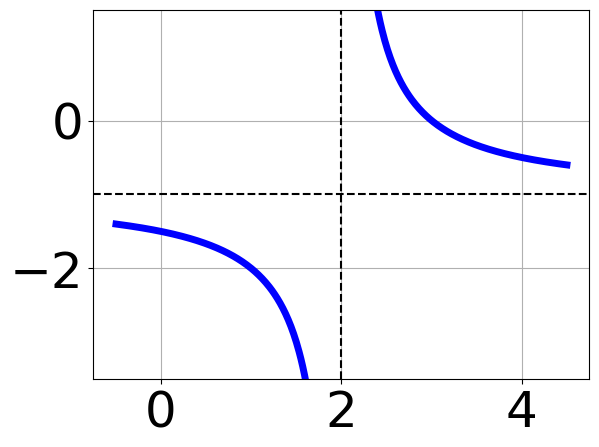
\includegraphics[width = 0.3\textwidth]{../Figures/rationalEquationToGraphAA.png}\item 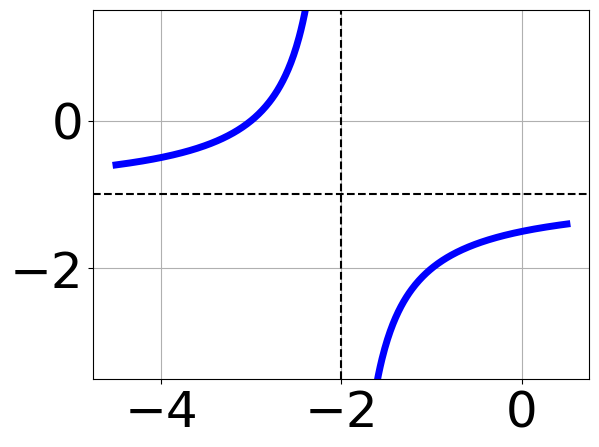
\includegraphics[width = 0.3\textwidth]{../Figures/rationalEquationToGraphBA.png}\item 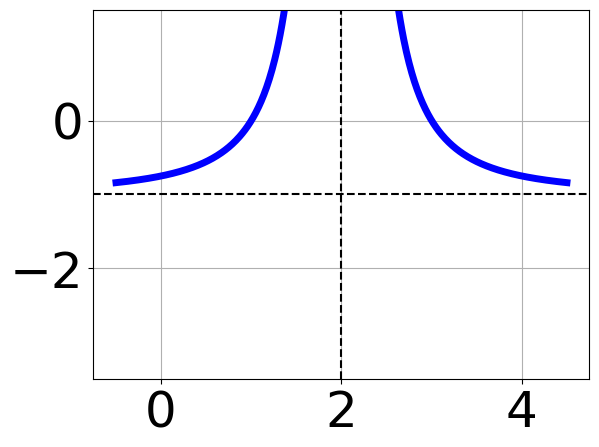
\includegraphics[width = 0.3\textwidth]{../Figures/rationalEquationToGraphCA.png}\item 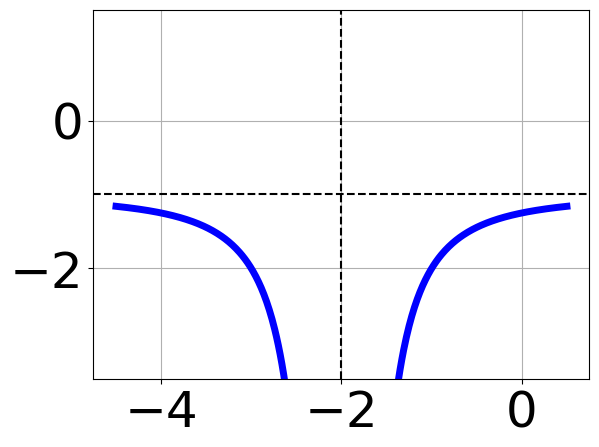
\includegraphics[width = 0.3\textwidth]{../Figures/rationalEquationToGraphDA.png}\end{multicols}\item None of the above.
\end{enumerate} }
\litem{
Choose the equation of the function graphed below.
\begin{center}
    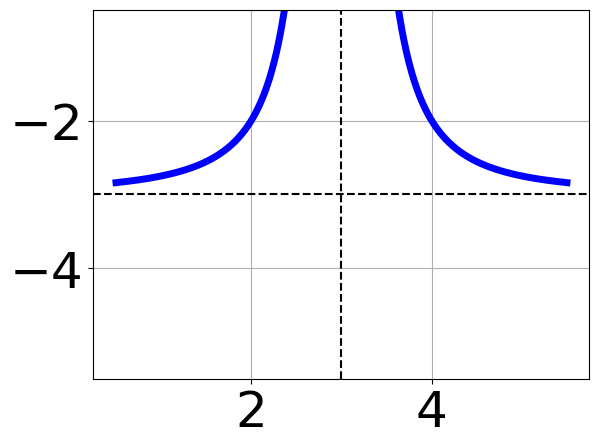
\includegraphics[width=0.5\textwidth]{../Figures/rationalGraphToEquationA.png}
\end{center}
\begin{enumerate}[label=\Alph*.]
\item \( f(x) = \frac{1}{x - 3} - 3 \)
\item \( f(x) = \frac{-1}{x + 3} - 3 \)
\item \( f(x) = \frac{-1}{(x + 3)^2} - 3 \)
\item \( f(x) = \frac{1}{(x - 3)^2} - 3 \)
\item \( \text{None of the above} \)

\end{enumerate} }
\litem{
Solve the rational equation below. Then, choose the interval(s) that the solution(s) belongs to.\[ \frac{-4x}{-7x + 4} + \frac{-6x^{2}}{-28x^{2} +37 x -12} = \frac{3}{4x -3} \]\begin{enumerate}[label=\Alph*.]
\item \( x \in [0.71,0.88] \)
\item \( x_1 \in [0.58, 0.67] \text{ and } x_2 \in [0.56,0.72] \)
\item \( \text{All solutions lead to invalid or complex values in the equation.} \)
\item \( x \in [0.8,0.93] \)
\item \( x_1 \in [0.58, 0.67] \text{ and } x_2 \in [0.73,1.12] \)

\end{enumerate} }
\litem{
Solve the rational equation below. Then, choose the interval(s) that the solution(s) belongs to.\[ \frac{7}{7x -3} + -6 = \frac{5}{-21x + 9} \]\begin{enumerate}[label=\Alph*.]
\item \( x \in [-0.26,-0.19] \)
\item \( x_1 \in [0.39, 0.58] \text{ and } x_2 \in [0.63,2.63] \)
\item \( \text{All solutions lead to invalid or complex values in the equation.} \)
\item \( x \in [0.63,1.63] \)
\item \( x_1 \in [-0.26, -0.19] \text{ and } x_2 \in [0.63,2.63] \)

\end{enumerate} }
\litem{
Choose the equation of the function graphed below.
\begin{center}
    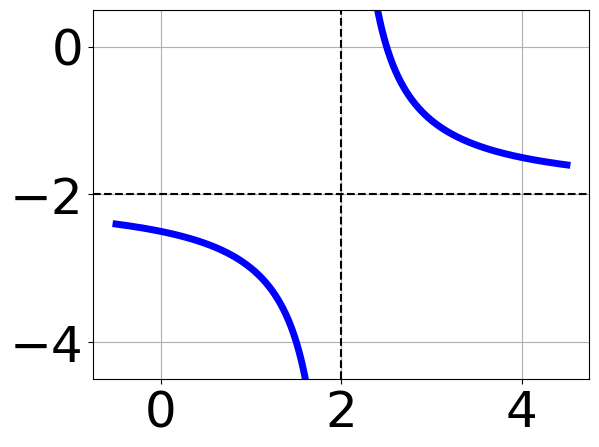
\includegraphics[width=0.5\textwidth]{../Figures/rationalGraphToEquationCopyA.png}
\end{center}
\begin{enumerate}[label=\Alph*.]
\item \( f(x) = \frac{1}{(x - 2)^2} - 2 \)
\item \( f(x) = \frac{-1}{x + 2} - 2 \)
\item \( f(x) = \frac{1}{x - 2} - 2 \)
\item \( f(x) = \frac{-1}{(x + 2)^2} - 2 \)
\item \( \text{None of the above} \)

\end{enumerate} }
\litem{
Solve the rational equation below. Then, choose the interval(s) that the solution(s) belongs to.\[ \frac{24}{48x + 18} + 1 = \frac{24}{48x + 18} \]\begin{enumerate}[label=\Alph*.]
\item \( x \in [-0.1,1] \)
\item \( \text{All solutions lead to invalid or complex values in the equation.} \)
\item \( x \in [-1.38,1.62] \)
\item \( x_1 \in [-0.5, -0.1] \text{ and } x_2 \in [-0.1,1.3] \)
\item \( x_1 \in [-0.5, -0.1] \text{ and } x_2 \in [-0.5,0.2] \)

\end{enumerate} }
\litem{
Choose the graph of the equation below.\[ f(x) = \frac{-1}{x + 2} - 1 \]\begin{enumerate}[label=\Alph*.]
\begin{multicols}{2}\item 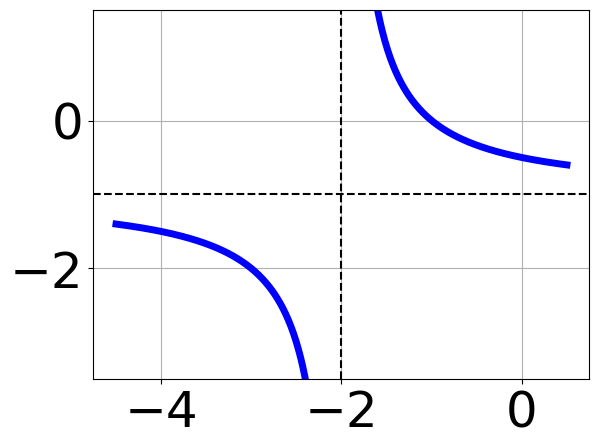
\includegraphics[width = 0.3\textwidth]{../Figures/rationalEquationToGraphCopyAA.png}\item 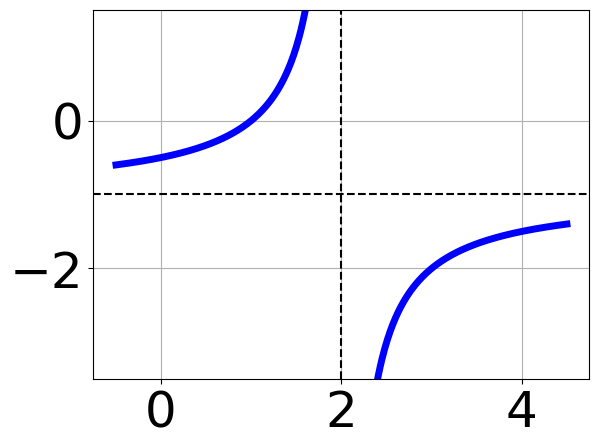
\includegraphics[width = 0.3\textwidth]{../Figures/rationalEquationToGraphCopyBA.png}\item 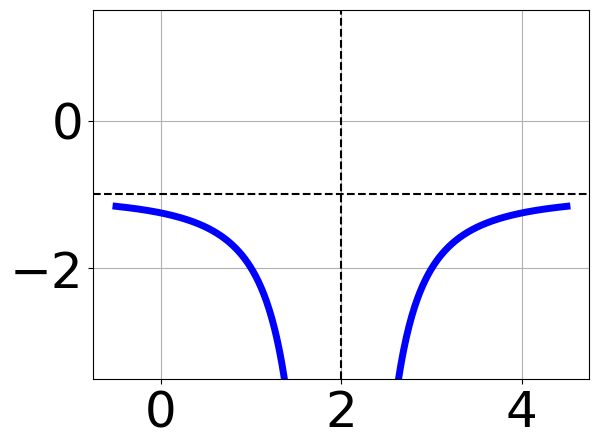
\includegraphics[width = 0.3\textwidth]{../Figures/rationalEquationToGraphCopyCA.png}\item 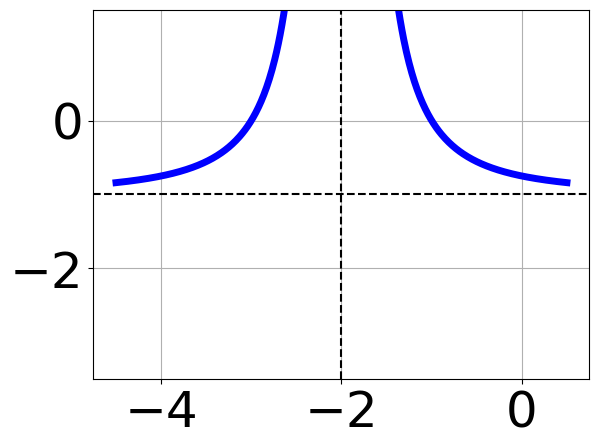
\includegraphics[width = 0.3\textwidth]{../Figures/rationalEquationToGraphCopyDA.png}\end{multicols}\item None of the above.
\end{enumerate} }
\litem{
Determine the domain of the function below.\[ f(x) = \frac{6}{20x^{2} -8 x -12} \]\begin{enumerate}[label=\Alph*.]
\item \( \text{All Real numbers except } x = a \text{ and } x = b, \text{ where } a \in [-17, -11] \text{ and } b \in [16, 17] \)
\item \( \text{All Real numbers except } x = a \text{ and } x = b, \text{ where } a \in [-1.6, 0.4] \text{ and } b \in [0, 6] \)
\item \( \text{All Real numbers except } x = a, \text{ where } a \in [-17, -11] \)
\item \( \text{All Real numbers.} \)
\item \( \text{All Real numbers except } x = a, \text{ where } a \in [-1.6, 0.4] \)

\end{enumerate} }
\litem{
Determine the domain of the function below.\[ f(x) = \frac{3}{25x^{2} -10 x -24} \]\begin{enumerate}[label=\Alph*.]
\item \( \text{All Real numbers except } x = a, \text{ where } a \in [-1.4, 0.4] \)
\item \( \text{All Real numbers except } x = a, \text{ where } a \in [-21, -19.1] \)
\item \( \text{All Real numbers except } x = a \text{ and } x = b, \text{ where } a \in [-1.4, 0.4] \text{ and } b \in [0.1, 2.7] \)
\item \( \text{All Real numbers except } x = a \text{ and } x = b, \text{ where } a \in [-21, -19.1] \text{ and } b \in [28.7, 30.2] \)
\item \( \text{All Real numbers.} \)

\end{enumerate} }
\litem{
Solve the rational equation below. Then, choose the interval(s) that the solution(s) belongs to.\[ \frac{3x}{-6x -4} + \frac{-7x^{2}}{-24x^{2} +2 x + 12} = \frac{4}{4x -3} \]\begin{enumerate}[label=\Alph*.]
\item \( x_1 \in [-1.55, -0.69] \text{ and } x_2 \in [-0.21,0.48] \)
\item \( x \in [0.45,0.96] \)
\item \( x \in [-0.84,-0.5] \)
\item \( \text{All solutions lead to invalid or complex values in the equation.} \)
\item \( x_1 \in [-0.84, -0.5] \text{ and } x_2 \in [0.56,0.89] \)

\end{enumerate} }
\end{enumerate}

\end{document}